\documentclass[14pt]{beamer}
\usetheme{Montpellier}
\usepackage[utf8]{inputenc}
\usepackage[english]{babel}
\usepackage{amsmath}
\usepackage{amsfonts}
\usepackage{amssymb}
\usepackage{graphicx}
\usepackage{enumitem}
\usepackage{lmodern}

\author{Oumaima Al Qoh, Francisco Arrieta, Lucia Camenisch, Manuela Giansante, Emily Schmidt, Camille Beatrice Valera}
\title{Case Study B \\ Pain Relief Medication}
\date{April 28, 2023} 
%\subject{}
%\logo{}
%\institute{}

  
\setbeamertemplate{navigation symbols}{
\usebeamerfont{footline}
\insertframenumber/\inserttotalframenumber
}



\begin{document}


\begin{frame}
\titlepage
\end{frame}



\begin{frame}
\frametitle{Table of Contents}
\tableofcontents
\end{frame}


\section{Case Statement}
\begin{frame}
\frametitle{Case Statement}
\begin{itemize}[label={$\blacktriangleright$}]
\item 20 experiments on mice with combinations of marijuana and morphine, of which:
\begin{itemize}[label={$\blacktriangleright$}]
\item 1 control experiment;
\item 5 experiments with marijuana only;
\item 8 experiments with morphine only;
\item 6 experiments with both drugs.
\end{itemize}
\item 10 mice used per experiment;
\item Each mouse undergoes a tail flick test.
\end{itemize}
\end{frame}

\begin{frame}
The tail flick test assesses the effect of drugs on the mouse.

\bigskip

In each experiment, the proportion of mice not flicking their tail can be interpreted as a \textbf{measure of the effect of the drug} for the chosen experimental dosage.
\end{frame}

\section{Objectives}
\begin{frame}
\frametitle{First Objective}
\textit{Determine the minimum dosage amount of the drugs that achieves \textbf{efficacy}.}

\bigskip

The dosage of a drug is said to be \textbf{efficient} if at least 50\% of the subjects are responding.
\end{frame}


\begin{frame}
\frametitle{Second Objective}
\textit{Detect whether a \textbf{synergy} exists between the two drugs.}

\bigskip

If the combined efficacy of the two drug dosages is greater than the sum of the individual efficacy of each drug for its respective dosage, there is \textbf{synergy}.
\end{frame}


\section{Identifying Synergy with the Isoboles Method}
\begin{frame}
\frametitle{Identifying Synergy with the Isoboles Method}
The isoboles method is a graphical representation which identifies synergy and helps to better understand the concept.
\end{frame}

\begin{frame}
\begin{center}
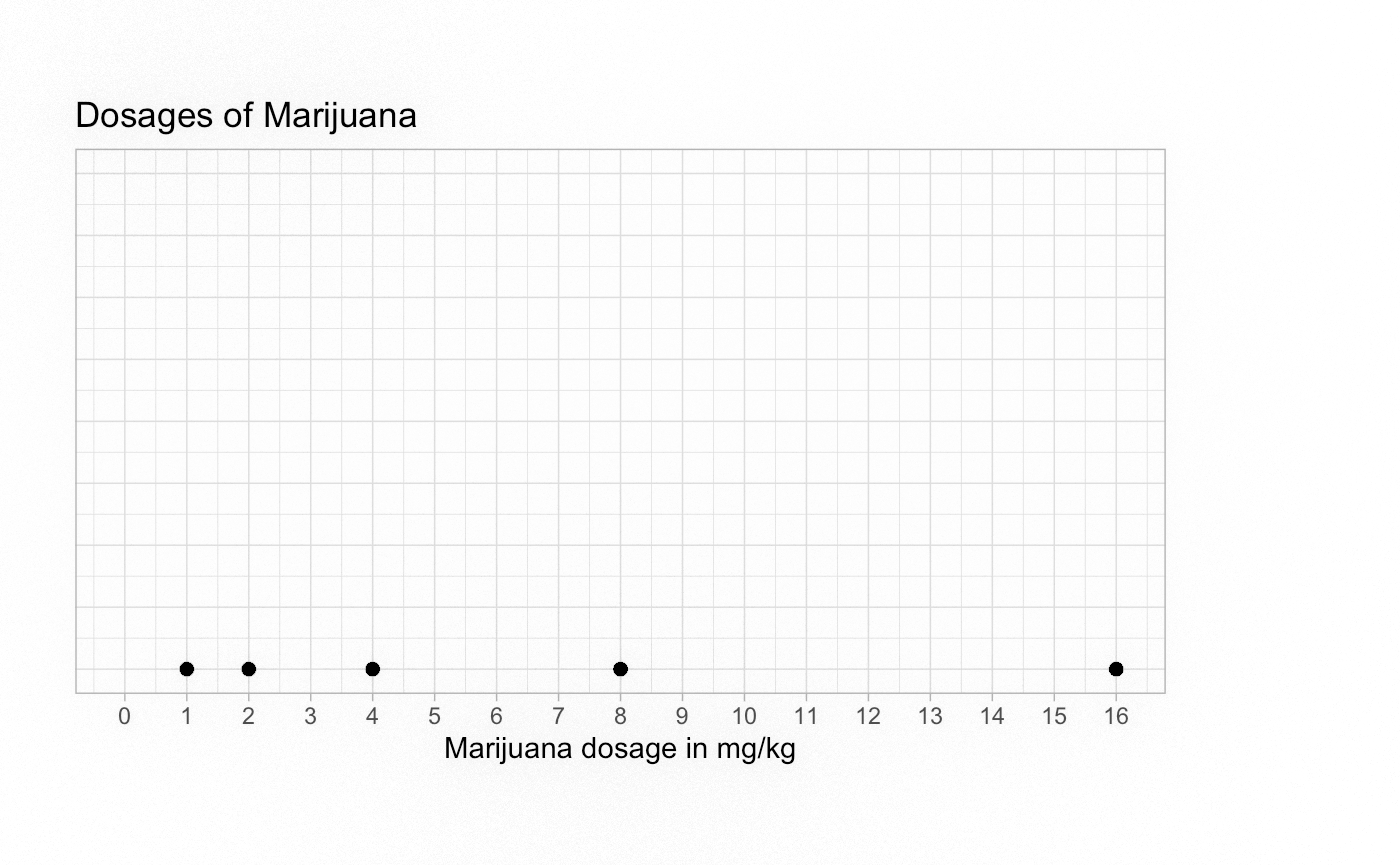
\includegraphics[scale=0.23]{img1.png}
\end{center}
\end{frame}

\begin{frame}
\begin{center}
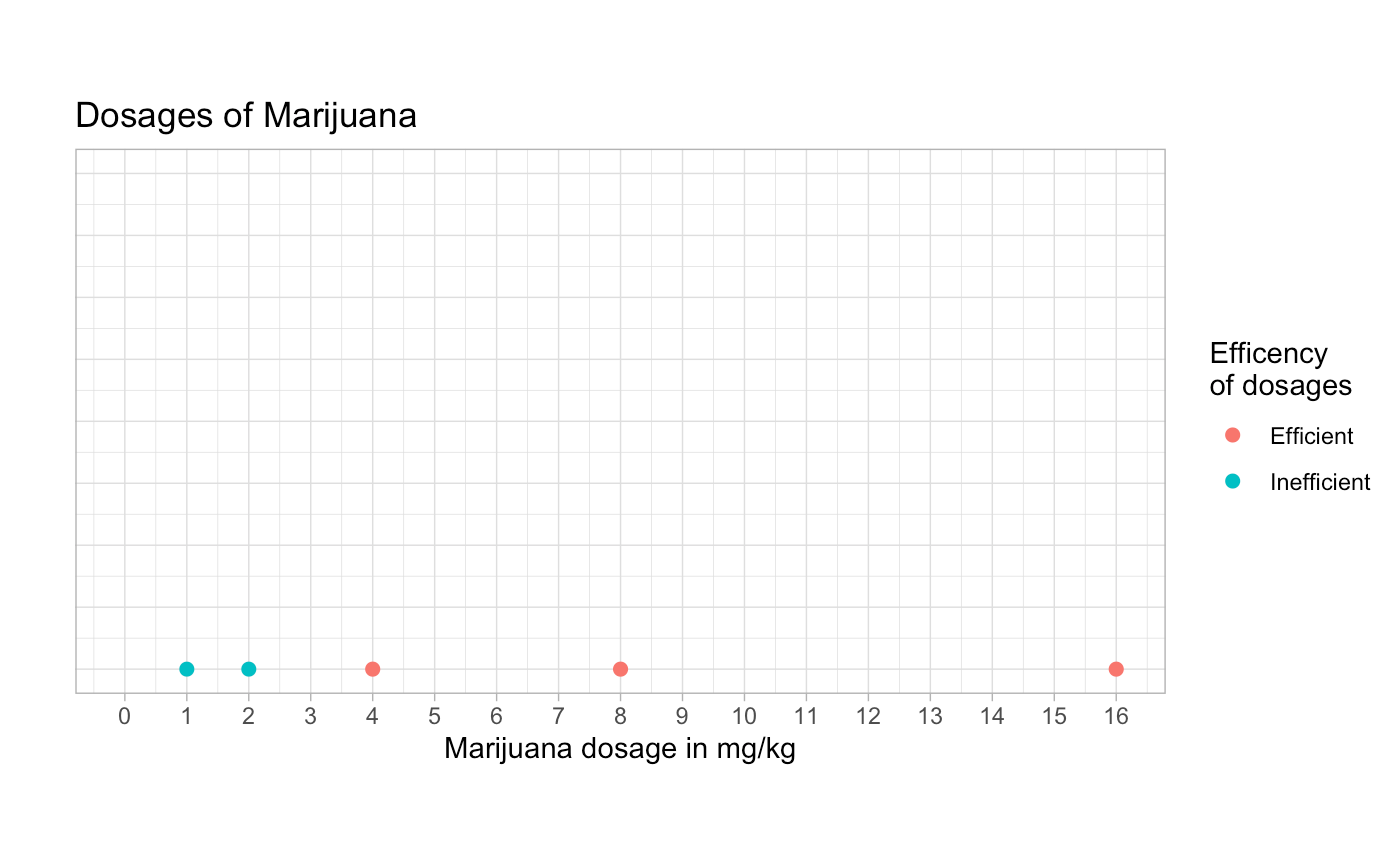
\includegraphics[scale=0.23]{img2.png}
\end{center}
\end{frame}

\begin{frame}
\begin{center}
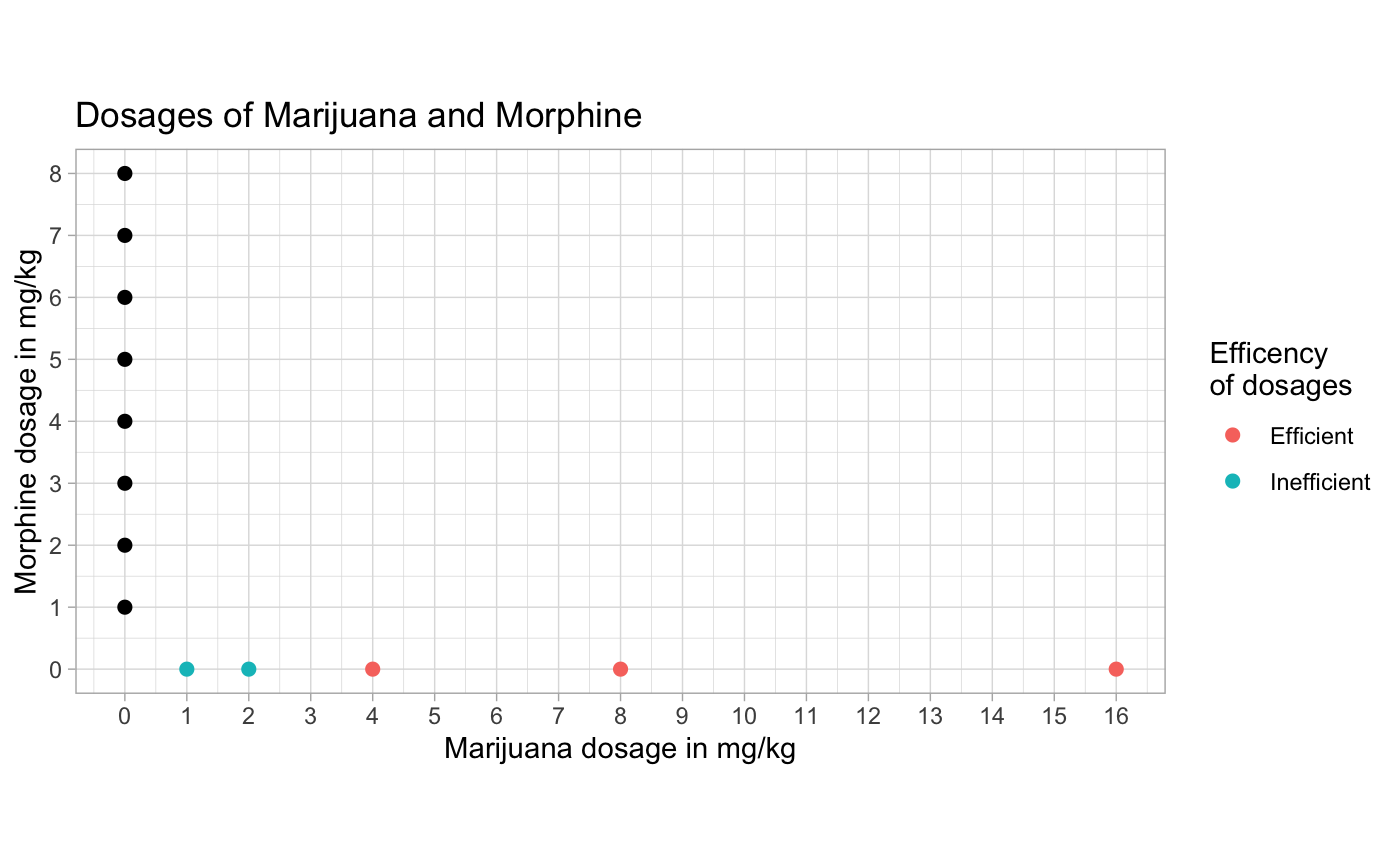
\includegraphics[scale=0.23]{img3.png}
\end{center}
\end{frame}

\begin{frame}
\begin{center}
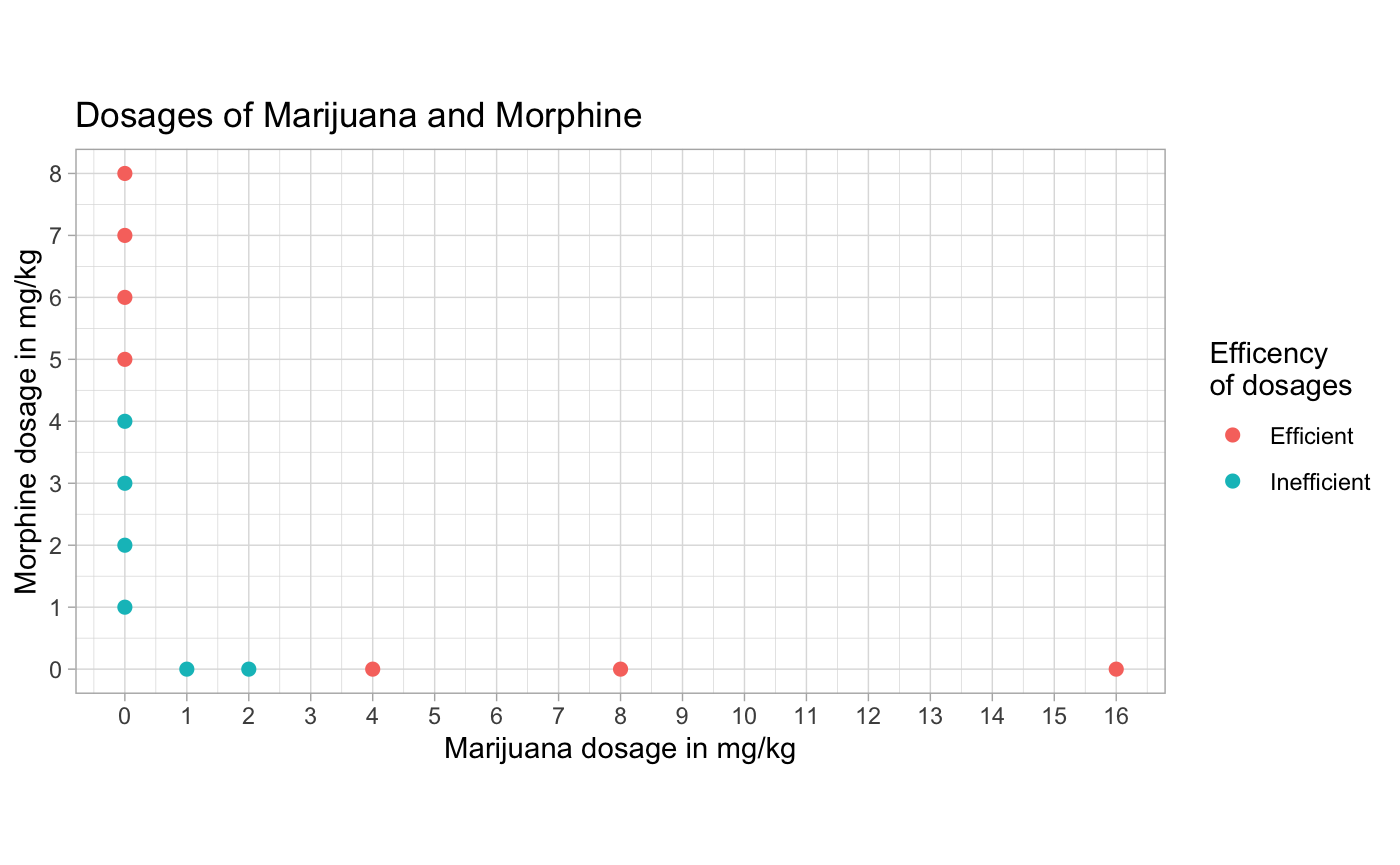
\includegraphics[scale=0.23]{img4.png}
\end{center}
\end{frame}

\begin{frame}
\begin{center}
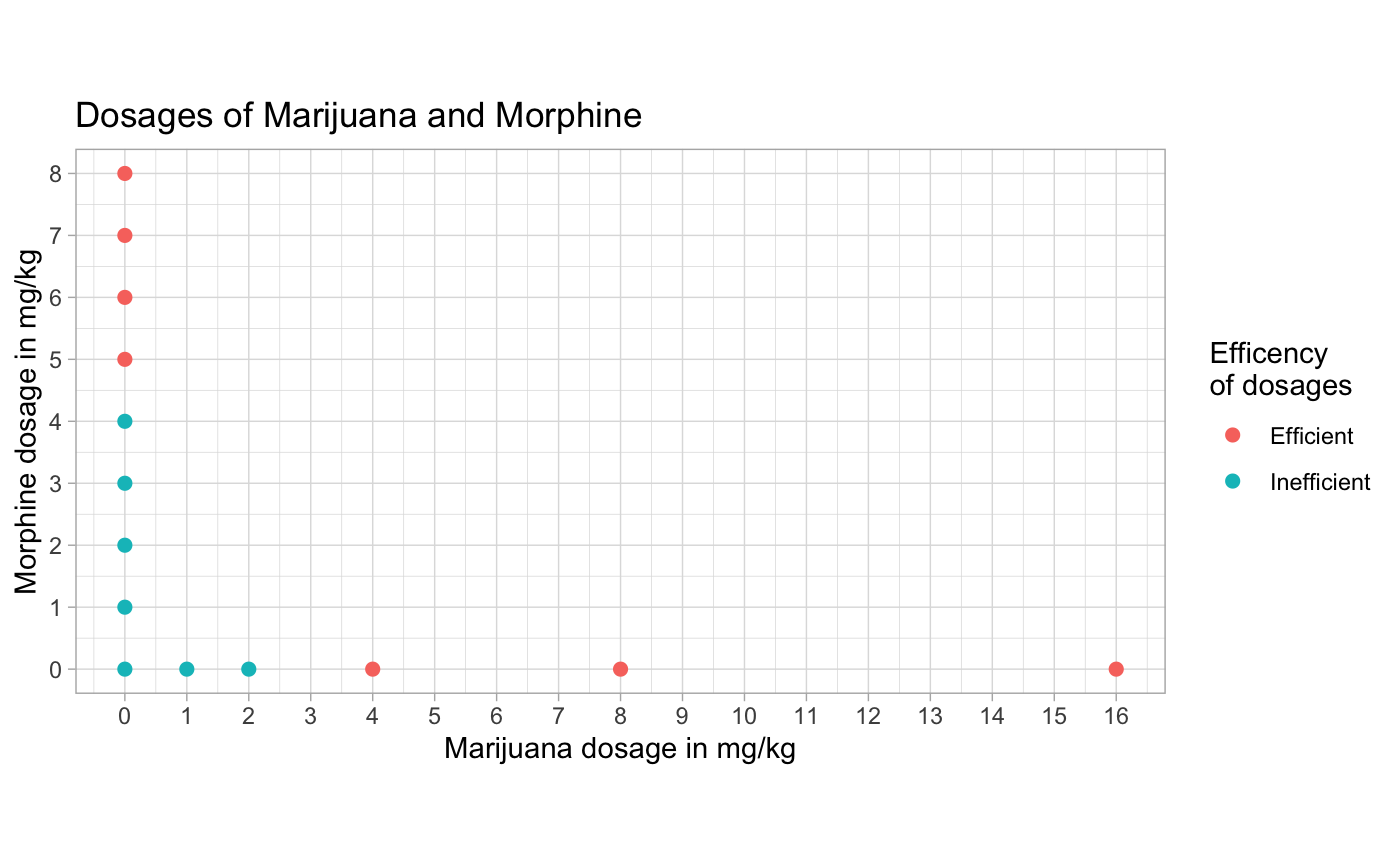
\includegraphics[scale=0.23]{img5.png}
\end{center}
\end{frame}

\begin{frame}
\begin{center}
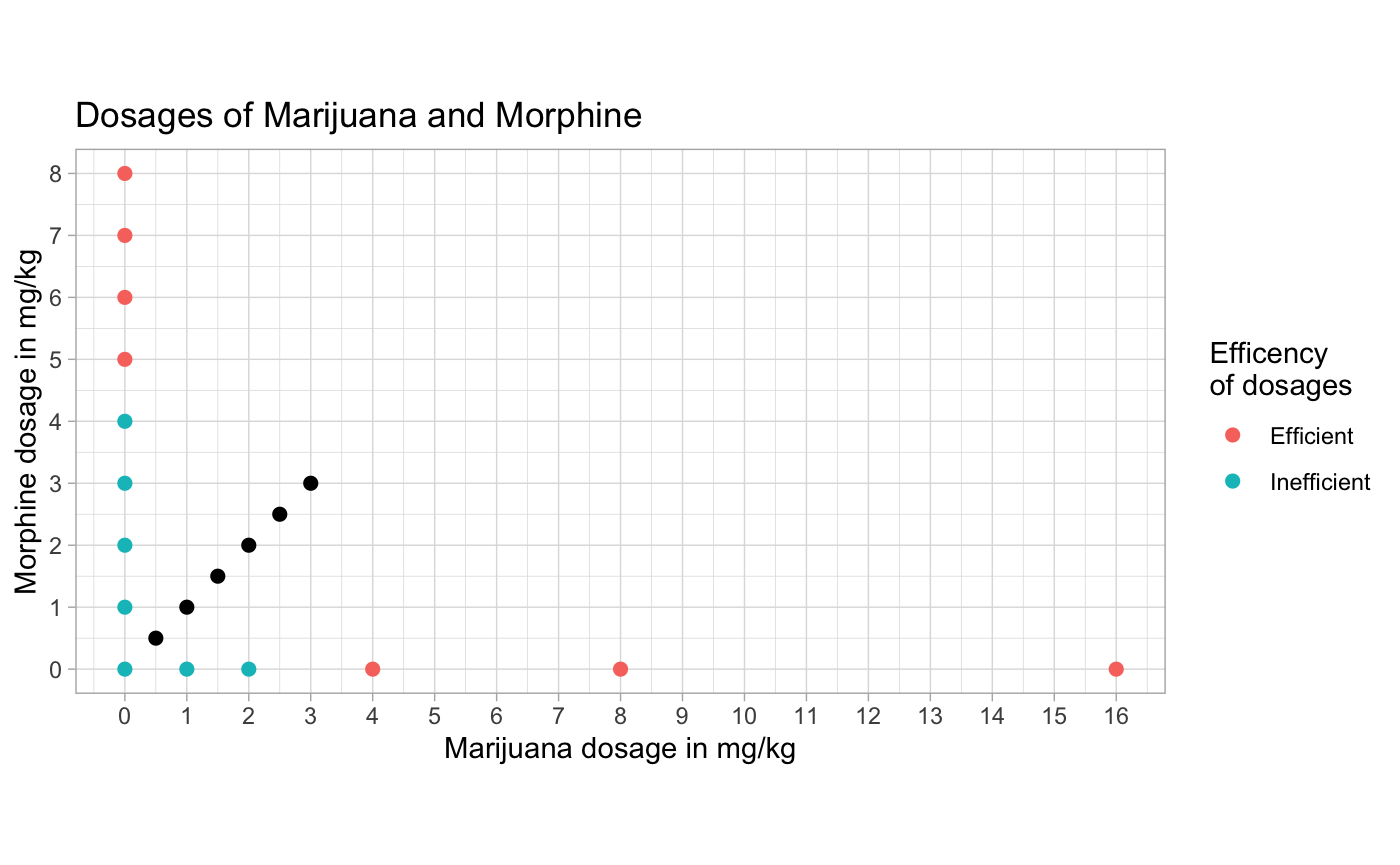
\includegraphics[scale=0.23]{img6.png}
\end{center}
\end{frame}

\begin{frame}
\begin{center}
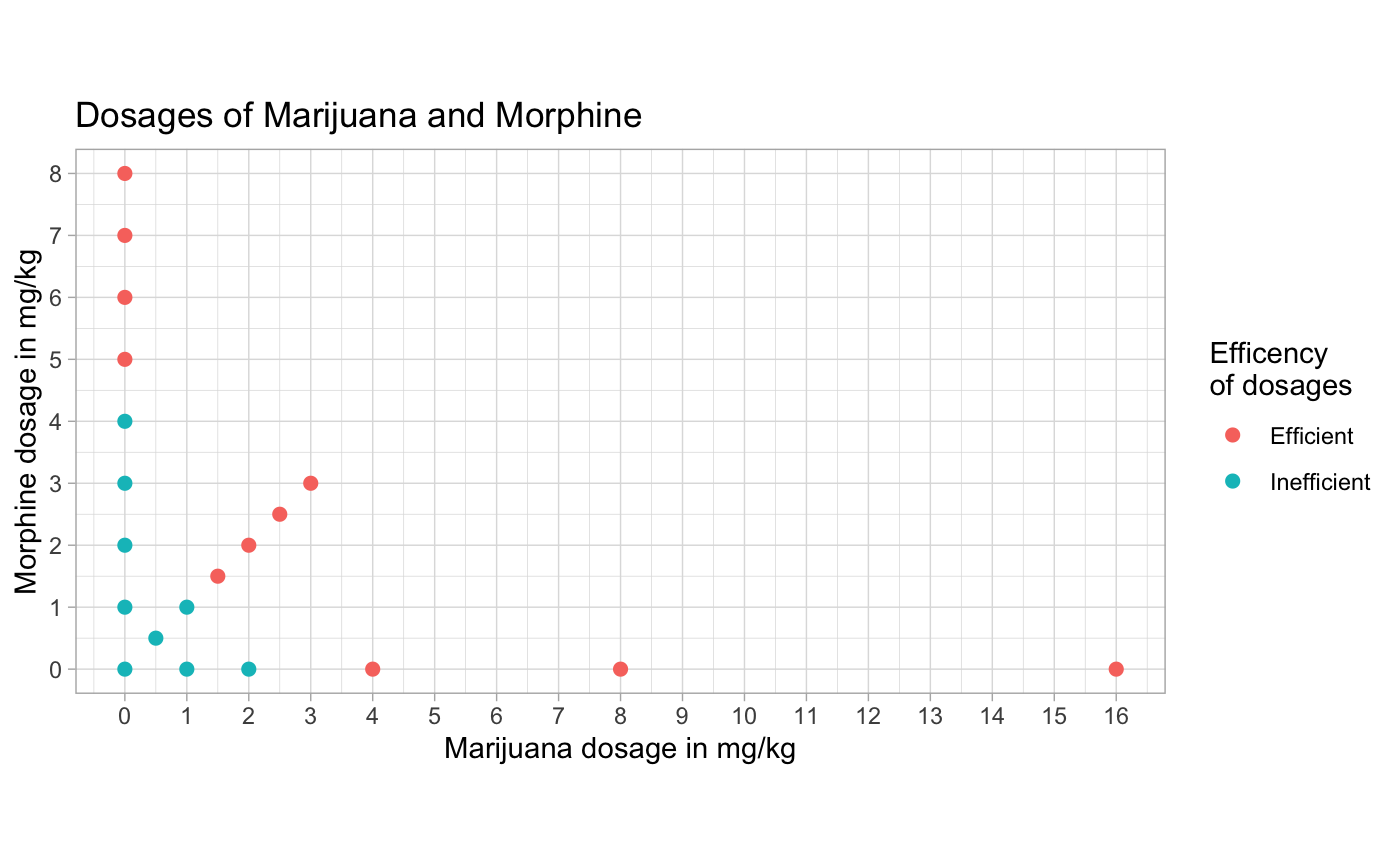
\includegraphics[scale=0.23]{img7.png}
\end{center}
\end{frame}

\begin{frame}
\begin{center}
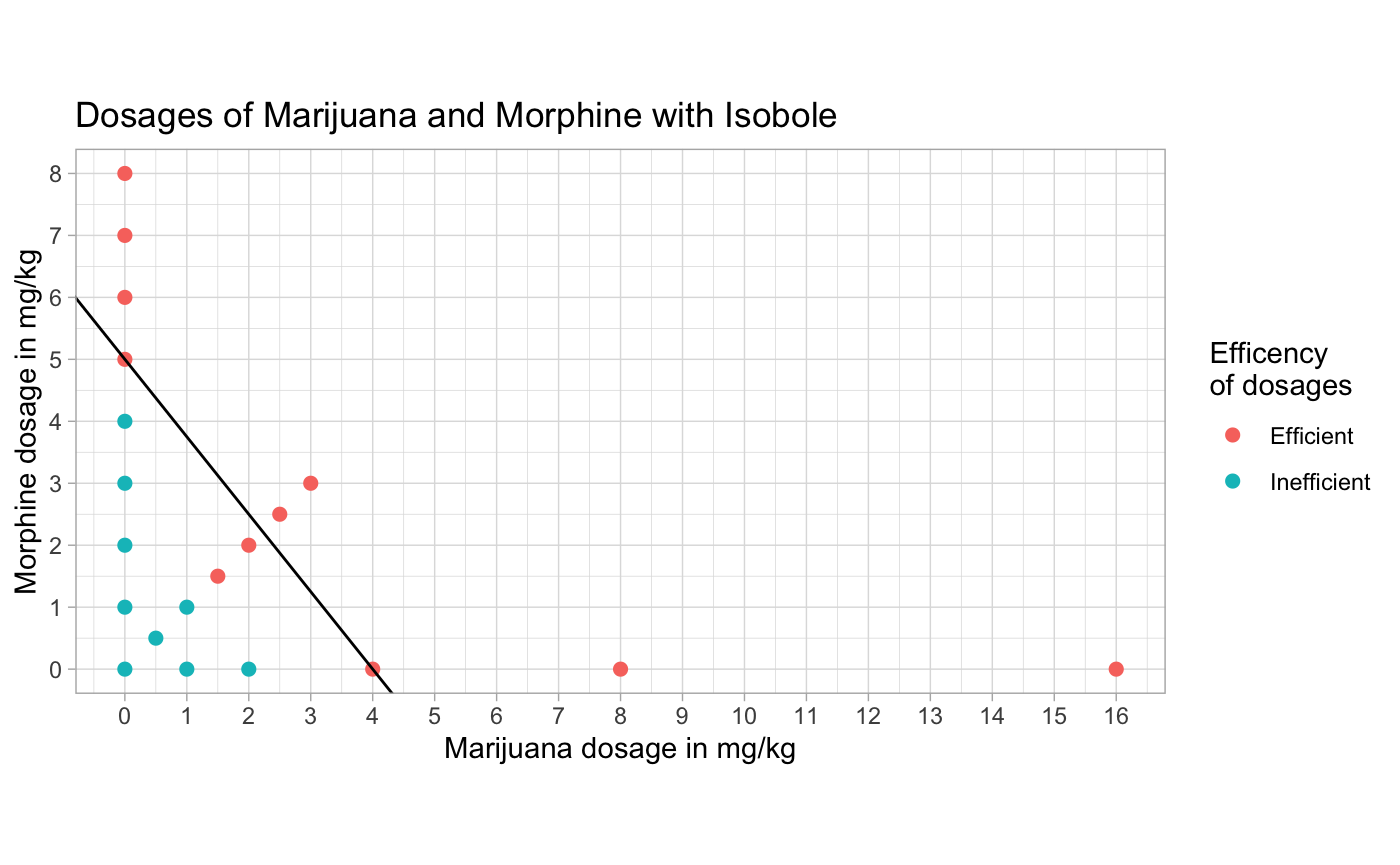
\includegraphics[scale=0.23]{img8.png}
\end{center}
\end{frame}

\section{Isobole Insights}
\begin{frame}
\frametitle{Isobole Insights}
\begin{itemize}[label={$\blacktriangleright$}]
\item Using 4 mg/kg of marijuana gives an equivalent effect ($\geq$ 50\% of mice responding) to using 5 mg/kg of morphine.
\item Combined dosages of the two drugs which are on the isobole have an equivalent effect to the ones mentioned above.
\item A combined dosage which is under the isobole but is still efficient is synergic.
\end{itemize}
\end{frame}

\section{Isobole Conclusion}
\begin{frame}
\frametitle{Isobole Conclusion}
\begin{itemize}[label={\checkmark}]
\item \textbf{First objective, minimal efficient dosage:} \\
\begin{itemize}[label={$\blacktriangleright$}]
\item 4.0 mg/kg for marijuana alone;
\item 5.0 mg/kg for morphine alone;
\item 1.5 mg/kg of each for both drugs.
\end{itemize}
\item \textbf{Second objective, synergy:} \\
Dosages of 1.5 mg/kg and 2.0 mg/kg each are synergic.
\end{itemize}
\end{frame}

\section{Isoboles Method Assumption}
\begin{frame}
\frametitle{Isoboles Method Assumption}
The ratio between dosages of morphine and marijuana when they give the same efficiency level is constant.
\end{frame}

\begin{frame}
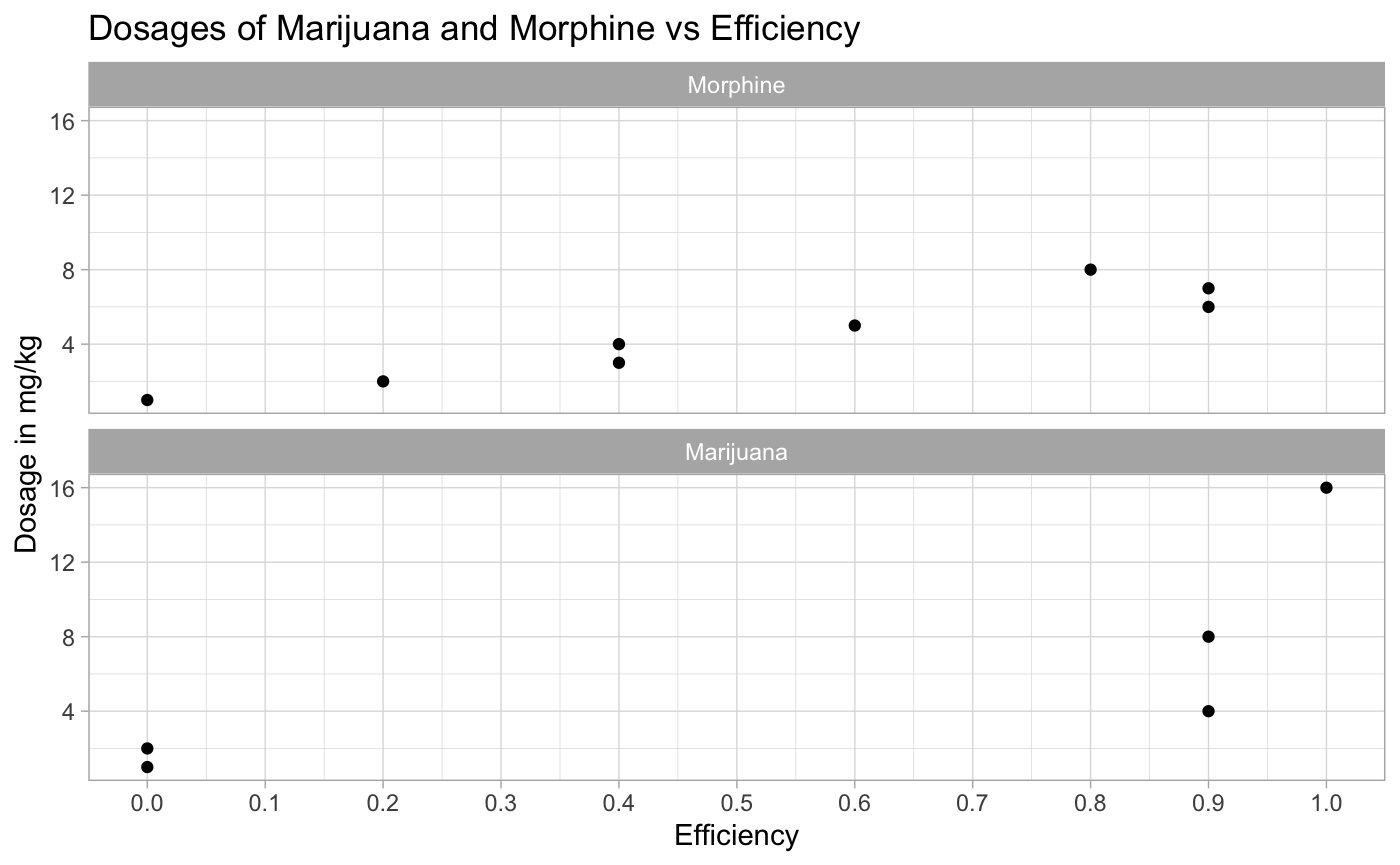
\includegraphics[scale=0.22]{dos_vs_eff.png}
\end{frame}

\begin{frame}
\begin{itemize}[label={$\blacktriangleright$}]
\item Only two common efficiency levels, 0.0 and 0.9
\item This is not enough to verify the assumption for this experiment.
\item This weakness is due to dosage choices for marijuana.
\item However, the linear isobole method is used in multiple experiments which are extremely similar.
\end{itemize}
\end{frame}

\section{Dosage Choices for Marijuana}

\begin{frame}
\frametitle{Dosage Choices for Marijuana}
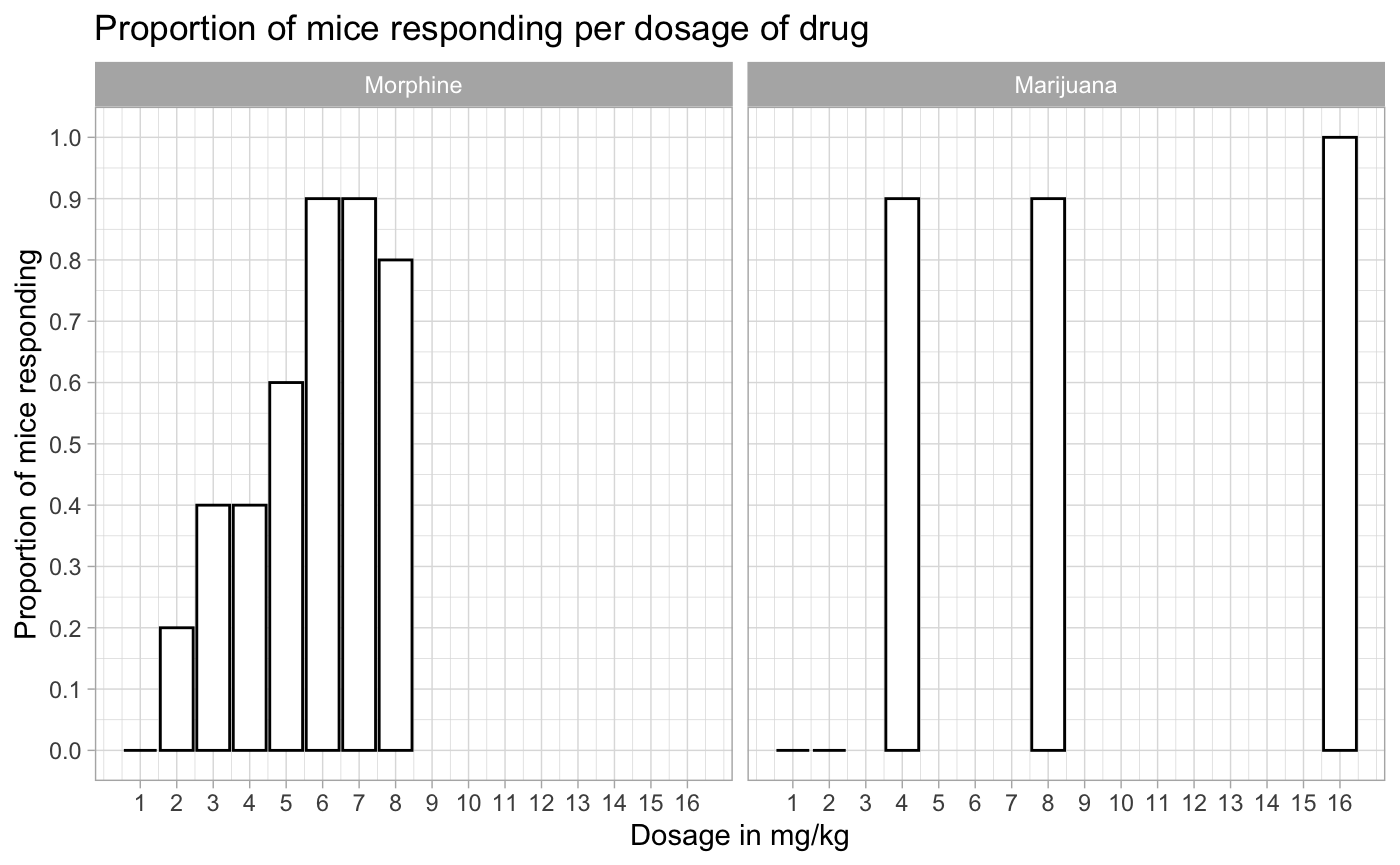
\includegraphics[scale=0.22]{prop_bar.png}
\end{frame}

\begin{frame}
\begin{itemize}[label={$\blacktriangleright$}]
\item The choice of dosages for marijuana does not allow for precise exploration of the minimal efficient dosage.
\item A better minimal efficient dosage could be found between 2.0 and 4.0 mg/kg.
\item This could change the isobole in a drastic way, making it stricter towards the synergic dosages.
\end{itemize}
\end{frame}

\begin{frame}
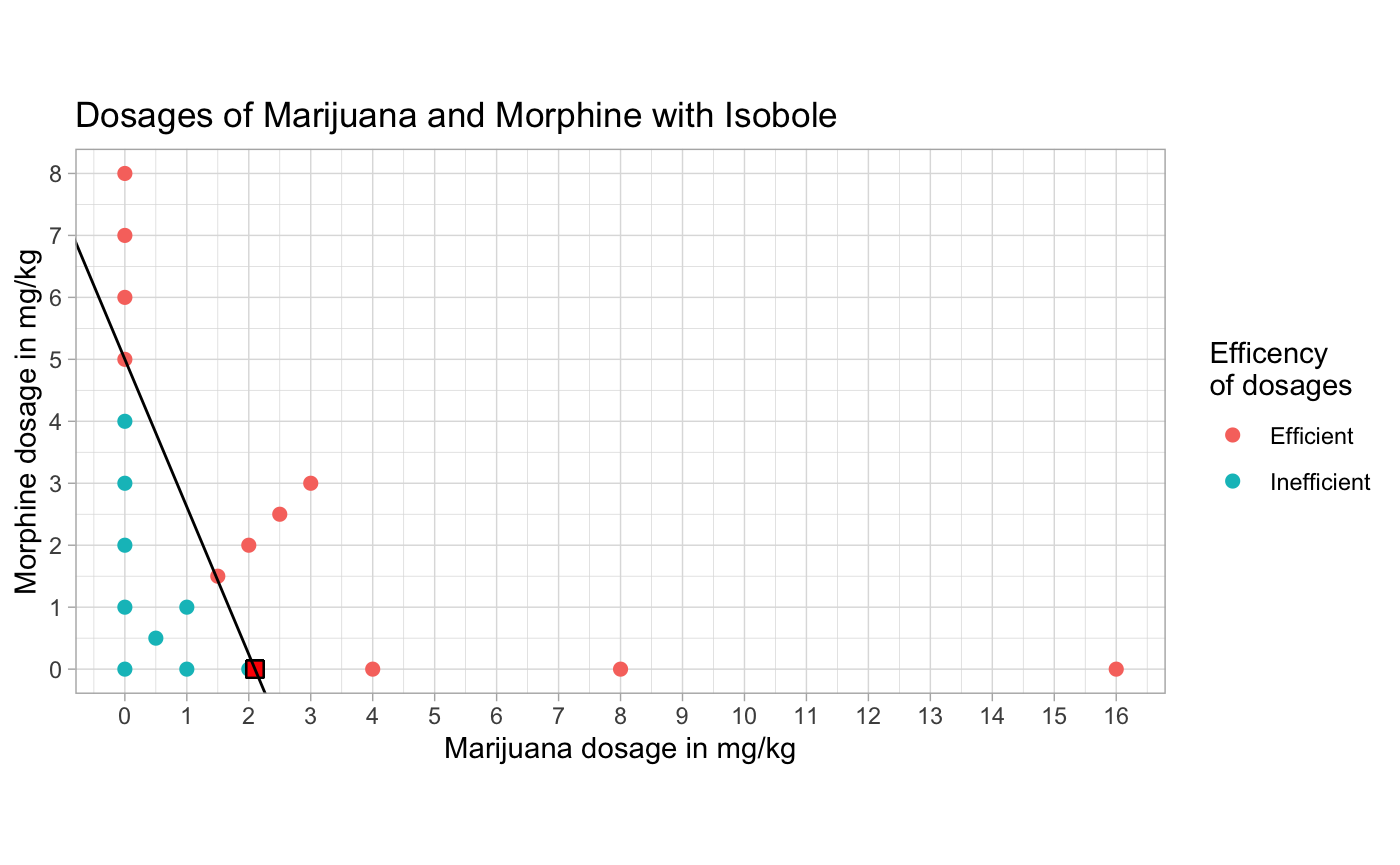
\includegraphics[scale=0.23]{mari_fake.png}
\end{frame}

\section{Recommendations}

\begin{frame}
\frametitle{Recommendations}
\begin{itemize}[label={\checkmark}]
\item \textbf{Complete the experiment with trials for at least 3 or 4 dosages of marijuana between 2.0 and 4.0 mg/kg.}
\item Experiment with more dosages of morphine between 4.0 and 5.0 mg/kg.
\item As of now, the best minimal efficient dosage is 1.5 mg/kg of marijuana and morphine combined.
\end{itemize}
\end{frame}

\begin{frame}
\frametitle{Q\&A Session}
Thank you for your attention. 

\bigskip

Feel free to ask us any question!
\end{frame}

\end{document}